Trong recommendation system có 2 thực thể chính là user và item. Mỗi user sẽ một độ quan tâm nhất định tới mỗi item. Mức độ quan tâm được gán cho một giá trị ứng với mỗi cặp user - item. Giả sử giá trị này được đo bằng giá trị user rate cho item, ta gọi giá trị này là rating. Khi đó, tập hệt các rating, bao gồm cả những giá trị chưa biết cần được dự đoán, được gọi là utility matrix.

Giả sử như ví dụ của utility matrix như hình dưới đây, user rate cho mỗi phim giá trị từ 1 đến 5, với 5 là rating tốt nhất. Khoảng trống thể hiện những phim mà user vẫn chưa rate. Những giá trị HP1, HP2, HP3 là phim Harry Potter 1, 2, 3, TW là Twilight, SW1, SW2, SW3 là Star Wars 1, 2, 3. User được thể hiện ở các chữ cái A đến D.

\begin{figure}[ht]
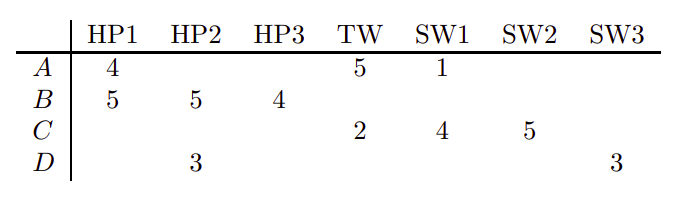
\includegraphics[width=\textwidth]{thesis/images/utility_matrix_2.png}
\caption{Utility Matrix}
\end{figure}

Thông thường, có rất nhiều user và item trong hệ thống, và mỗi user chỉ rate một số lượng ít các item hay không rate item nào. Do vậy trong utility matrix thường rất nhiều ô trống và những ô được điền là rất ít.

Rõ ràng càng nhiều ô được điền thì độ chính xác của hệ thống sẽ càng được cải thiện. Vì vậy các hệ thống luôn hỏi người dùng về sự quan tâm của họ tới sản phẩm, và muốn người dùng đánh giá càng nhiều sản phẩm càng tốt. Việc đánh giá sản phẩm không những giúp các người dùng khác biết được chất lượng sản phẩm mà còn giúp hệ thống biết được sở thích của người dùng, qua đỡ có thể quảng cáo hợp lý.

Nếu không có utility matrix thì gần như không thể gợi ý sản phẩm cho người dùng. Do vậy việc xây dựng utility matrix là việc rất quan trọng. Có 2 hướng tiếp cận phổ biến để xác định giá trị rating cho mỗi cặp user-item trong utility matrix. 

Hướng thứ nhất là nhờ người dùng rate sản phẩm. Ví dụ như Amazon luôn nhờ người dùng rate các sản phẩm của họ bằng việc gửi các email nhắc nhở. Nhiều hệ thống khác cũng áp dụng cách này. Tuy nhiên phương pháp này có một vài hạn chế vì thường người dùng ít khi rate sản phẩm. Và những rate đó có thể là đánh giá thiên lệch của người rate.

Hướng thứ hai là dựa vào hành vi của user. Ví dụ, nếu một người xem 1 bộ phim trên netflix, hay 1 clip trên youtube hay là mua 1 sản phẩm trên Amazon chứng tỏ người dùng thích sản phẩm đó. Youtube dựa trên những video mà người dùng đã xem để recommend cho người dùng những video khác liên quan tới những video đã xem đó. Thường thì với phương pháp này, chỉ có thể xây dựng utility matrix với giá trị 0 và 1. Trong đó, 0 thể hiện việc chưa có thông tin và 1 thể hiện việc đã xem video (thích sản phẩm). Tuy nhiên, cũng có thể xây dựng ma trận có giá trị cao hơn 1 tùy thuộc vào số lần người dùng xem video đó hay là thời gian xem video đó. Nút dislike cũng mang lại giá trị đánh giá vì thể hiện việc người dùng không thích video, ví dụ có thể gán giá trị -1 trong utility matrix.